\monster{Arimán}{4}{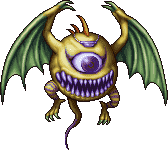
\includegraphics[width=0.21\textwidth]{./art/monsters/ahriman.png}}
{
 PV: & \hfill 28 & PM: & \hfill 24\\
 FUE: & \hfill 0 & DEF: & \hfill 1 \\
 MAG: & \hfill 4 & RES: & \hfill 4 \\
 AGI: & \hfill 4 & Tamaño: & \hfill P\\
}
{
 \textbf{Rayo}: 2d de daño, 3u Alcance \hfill \textbf{Botín:} 350 Gil 
 
 \mtech{Onda Espeluznante}{6}{1t}{Único}{3u}{
 El objetivo hace una tirada con DC 8. Si falla, sufre 2d de daño y queda en \hyperlink{status}{Silencio} por 3 turnos. }{\silence} 
 %\vspace{0.1cm} \hrule \vspace{0.1cm} 
 %\emph{"¡Ningún ser de toda la creación puede detenerme! ¡Ustedes también caerán ante mi!" -- Arimán} 
}